\documentclass[12pt, twoside]{article}
\usepackage[letterpaper, margin=1in, headsep=0.5in]{geometry}
\usepackage[english]{babel}
\usepackage[utf8]{inputenc}
\usepackage{amsmath}
\usepackage{amsfonts}
\usepackage{amssymb}
\usepackage{tikz}
\usepackage{yhmath}
%\usetikzlibrary{quotes, angles}

\usepackage{graphicx}
\usepackage{enumitem}
\usepackage{multicol}

\usepackage{fancyhdr}
\pagestyle{fancy}
\fancyhf{}
\renewcommand{\headrulewidth}{0pt} % disable the underline of the header

\fancyhead[RE]{\thepage}
\fancyhead[RO]{\thepage \\ Name: \hspace{3cm}}
\fancyhead[L]{BECA / Dr. Huson / 10th Grade Geometry\\* 4 April 2019}

\begin{document}
\subsubsection*{9.5 Do Now: Areas and volumes}
 \begin{enumerate}


\item Find the area of $\triangle ABC$,  $Area= \frac{1}{2}bh$. The altitude $h$ of the triangle is 5 centimeters and the base $AB=9.25$ cm.\\[1cm]
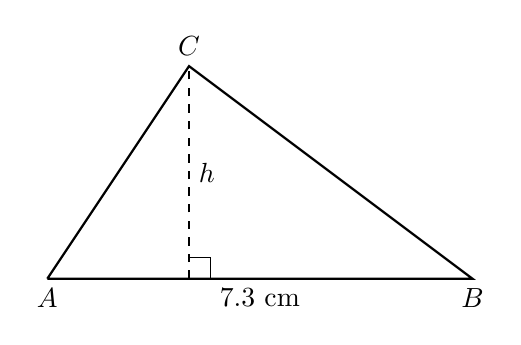
\begin{tikzpicture}[scale=0.9]
  \draw [thick]
    (2,0)node[below]{$A$}--
    (8,0)node[below]{$B$}--
    (4,3)node[above]{$C$} --(2,0);
 \draw [dashed] (4,0)--(4,3);
 \draw (4,0)++(0.3,0)--++(0,0.3)--+(-0.3,0);
 \node at (4,1.5)[right]{$h$};
 \node at (5,0)[below]{$7.3$ cm};
\end{tikzpicture}

 \vspace{1.5cm}

\item The figure shows a rectangle 3 cm wide and 2 cm high.
  \begin{center}
    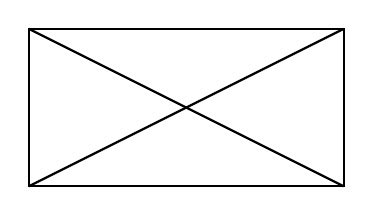
\begin{tikzpicture}%[scale=0.9]
      \coordinate (A) at (0, 0); %[label=above left:$P$]
      \coordinate (B) at (4, 0);
      \coordinate (C) at (4, 2);
      \coordinate (D) at (0, 2);
      \draw [thick] (A)--(B)--(C)--(D)--cycle;
      \draw [thick] (A)--(C);
      \draw [thick] (B)--(D);
      %\draw [thick, xshift=2cm, yshift=2.5cm] (85:3);
    \end{tikzpicture}
  \end{center}
    \begin{enumerate}
      \item What is the area of the rectangle? \vspace{2.5cm}
      \item What is the perimeter of the rectangle? \vspace{2.5cm}
      \item The rectangle is divided by its diagonals into four triangles? Which triangles are larger, or are they all the same size? Justify your response. \vspace{2cm}
    \end{enumerate}

\newpage

\item Circle $O$ has a diameter $\overline{AB}$, as shown.
  \begin{enumerate}
    \item Given that $m \wideparen{BC}=50^\circ$. Find $m\angle A$. \vspace{1cm}
    \item Write down $m \wideparen{ADB}$.  \vspace{1cm}
    \item Find $m\angle C$.
  \end{enumerate}
      \begin{center}
      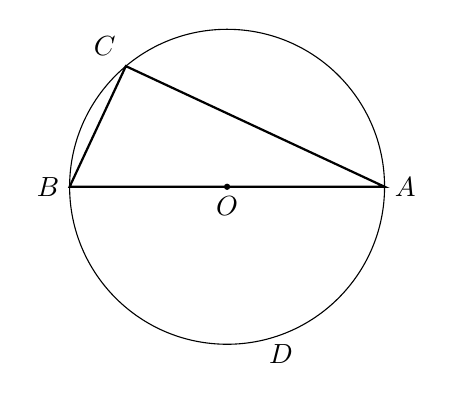
\begin{tikzpicture}[scale=.4]
        \draw (0,0) circle[radius=5];
        \draw [thick]
        (0:5) node[right] {$A$}--
        (180:5) node[left] {$B$}--
        (130:5) node[above left] {$C$}--cycle;
        \fill (0,0) circle[radius=0.1] node[below]{$O$};
        %\draw (75:1.8) node[above] {$C$};
        \draw (290:5) node[below] {$D$};
      \end{tikzpicture}
    \end{center}

  \item In right triangle $ABC$ shown below, point $D$ is on $\overline{AB}$ and point $E$ is on $\overline{BC}$ such that $\overline{AC} \parallel \overline{DE}$. Given $BD=12$, $BC=12$, and $EC=2$.
    \begin{center}
      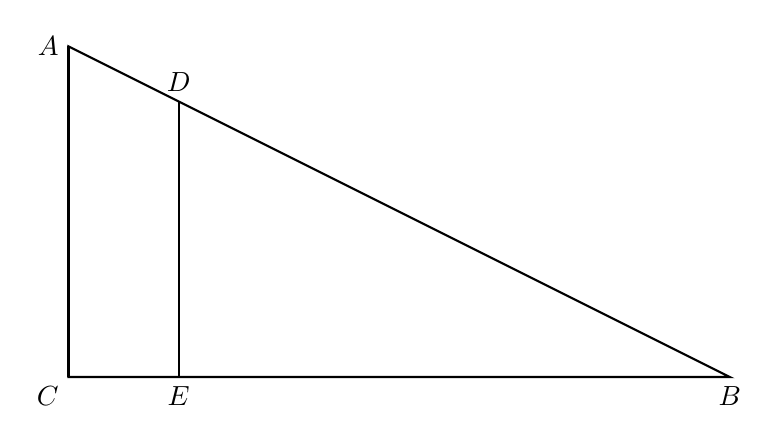
\begin{tikzpicture}[scale=0.7]
        \coordinate [label=left:$A$](A) at (-12,6);
        \coordinate [label=below:$B$](B) at (0, 0);
        \coordinate [label=below left:$C$](C) at (-12,0);
        \coordinate [label=above:$D$](D) at (-10, 5);
        \coordinate [label=below:$E$](E) at (-10,0);
        \draw [thick] (A)--(B)--(C)--cycle;
        \draw [thick] (A)--(C);
        \draw [thick] (D)--(E);
      \end{tikzpicture}
    \end{center}
   \begin{enumerate}
     \item Find the length of $\overline{BE}$. \vspace{0.5cm}
     \item Find the scale factor, $k$, dilating $\triangle DBE \rightarrow \triangle ABC$, centered at $B$. \vspace{1.5cm}
     \item Find $AD$.
    \end{enumerate}


\end{enumerate}
\end{document}
